%; whizzy chapter -dvi
% -initex iniptex -latex platex -format platex -bibtex jbibtex -fmt fmt
% 以上 whizzytex を使用する場合の設定。
 
%     Tokyo Debian Meeting resources
%     Copyright (C) 2012 Junichi Uekawa
%     Copyright (C) 2011, 2015 Nobuhiro Iwamatsu

%     This program is free software; you can redistribute it and/or modify
%     it under the terms of the GNU General Public License as published by
%     the Free Software Foundation; either version 2 of the License, or
%     (at your option) any later version.

%     This program is distributed in the hope that it will be useful,
%     but WITHOUT ANY WARRANTY; without even the implied warranty of
%     MERCHANTABILITY or FITNESS FOR A PARTICULAR PURPOSE.  See the
%     GNU General Public License for more details.

%     You should have received a copy of the GNU General Public License
%     along with this program; if not, write to the Free Software
%     Foundation, Inc., 51 Franklin St, Fifth Floor, Boston, MA  02110-1301 USA

%  preview (shell-command (concat "evince " (replace-regexp-in-string "tex$" "pdf"(buffer-file-name)) "&"))

%%ここからヘッダ開始。

\documentclass[mingoth,a4paper]{jsarticle}
\usepackage{monthlyreport}
% 日付を定義する、毎月変わります。
\newcommand{\debmtgyear}{2017}
\newcommand{\debmtgmonth}{4}
\newcommand{\debmtgdate}{22}
% started from zero:
% (let ((year 2013) (month 7)) (+ (* (- year 2005) 12) month -1))
\newcommand{\debmtgnumber}{150}

% tikz picture の為のマクロ設定
\usepackage[dvipdfmx]{graphicx}
\usepackage{tikz}

\begin{document}

\begin{titlepage}
\thispagestyle{empty}
% タイトルページ:編集必要な部分は最初のマクロに飛ばすこと

\vspace*{-2cm}
第\debmtgnumber{}回 東京エリア Debian 勉強会資料\\
\hspace*{-2cm}
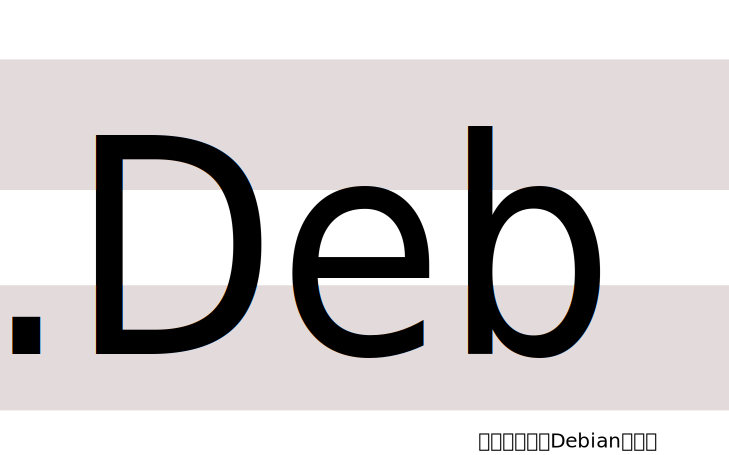
\includegraphics{image2012-natsu/dotdeb.pdf}\\
\hfill{}\debmtgyear{}年\debmtgmonth{}月\debmtgdate{}日

% ここはアップデートすること
% 全角文字にしないとフォントのサイズが合わないので注意
\rotatebox{10}{\fontsize{30}{30} {\gt 特集 :パッケージカスタマイズ}}\\

\vspace*{-2cm}
\hfill{}\includegraphics[height=6cm]{image200502/openlogo-nd.eps}
\end{titlepage}

\newpage

\begin{minipage}[b]{0.2\hsize}
 \definecolor{titleback}{gray}{0.9}
 \colorbox{titleback}{\rotatebox{90}{\fontsize{80}{80} {\gt デビアン勉強会} }}
\end{minipage}
\begin{minipage}[b]{0.8\hsize}
\hrule
\vspace{2mm}
\hrule
\begin{multicols}{2}
\tableofcontents
\end{multicols}
\vspace{2mm}
\hrule
\end{minipage}

\dancersection{最近のDebian関連のミーティング報告}{杉本 典充}

\subsection{第148回東京エリアDebian勉強会}

2017年2月11日(土)に第148回東京エリアDebian勉強会を開催しました。会場は銀座にある朝日ネットさんをお借りして行いました。参加者は9名でした。

2017年2月5日にDebian 9 stretchのFull Freeze宣言がアナウンスされました\footnote{\url{https://lists.debian.org/debian-devel-announce/2017/02/msg00001.html}}。今回の勉強会では、リリースクリティカルバグを解決するべく作業を行う「バグ・スカッシュ・パーティー」を行いました。

Debian Developerである岩松さんからリリースクリティカルバグの調べ方、patchの投稿作法、BTSへのタグの効果的なつけ方を参加者へ共有しました。その後、リリースクリティカルバグの中で難易度の高いものと低いものを選別し、参加者は解決できるものからバグ解決に臨みました。

バグ・スカッシュ・パーティの結果は、以下のDebian wikiにまとめています。

\url{https://wiki.debian.org/BSP/2017/02/jp/Tokyo}


\subsection{OSC 2017 Tokyo/Spring 出展(第149回東京エリアDebian勉強会)}

2017年3月11日(土)に開催されたOSC 2017 Tokyo/Springへ、東京エリアDebian勉強会/DebianJPとして出展しました。

展示ブースではDebian GNU/LinuxをインストールしたPC及びARMとFPGAの両方を搭載したリファレンスボードの展示、Debian Projectと東京エリアDebian勉強会の広報活動を行いました。また、OSC参加者と交流を深めました。

セミナーは「第149回東京エリアDebian勉強会」として開催し、「Debian updates」という表題で岩松さんが発表しました。また、セミナーに参加した25名の方々から疑問や質問に回答しました。


\dancersection{事前課題}{杉本 典充}

今回の事前課題は以下です:
\begin{enumerate}
  \item Hack Timeは何をしますか。
  \item 普段使っているDebianパッケージのうち、カスタマイズ(コンパイルオプション変更や独自修正など)しているものがあれば、そのパッケージ名とカスタマイズ内容を書いてください。
\end{enumerate}
この課題に対して提出いただいた内容は以下です。
\begin{multicols}{2}
{\small
\begin{prework}{ dictoss }
  \begin{enumerate}
  \item RFAになっているsnmpttのupstreamおよびパッケージの中身の調査
  \item backportsで問題ないため、既存パッケージのカスタマイズはしていない。
  \end{enumerate}
\end{prework}

\begin{prework}{ Roger Shimizu }
  \begin{enumerate}
  \item パッケージメインテインとか、バグ潰しなどするつもり
  \item 現在特にありません
  \end{enumerate}
\end{prework}

\begin{prework}{ hatochan }
  \begin{enumerate}
  \item debianインストールまたはlive-helpをごにょごにょ
  \item firmware関連のパッケージを試行錯誤
  \end{enumerate}
\end{prework}

\begin{prework}{ kenhys }
  \begin{enumerate}
  \item パッケージのメンテナンス
  \item 独自にメンテするのが面倒なので基本はしない 必要ならフィードバックしてパッケージ側に反映してもらう
  \end{enumerate}
\end{prework}

\begin{prework}{ Marc Dequènes (Duck) }
  \begin{enumerate}
  \item BSPとかメンター作業など
  \item backportとかpending fixなどのためにカスタマイズをよくします。
  \end{enumerate}
\end{prework}

\begin{prework}{ koedoyoshida }
  \begin{enumerate}
  \item Debian関係作業、PyConJP関係作業
  \item 最近は無し
  \end{enumerate}
\end{prework}

}
\end{multicols}

\dancersection{Debian Trivia Quiz}{杉本 典充}

Debianの昨今の話題についてのQuizです。

今回の出題範囲は\url{debian-devel-announce@lists.debian.org} や \url{debian-news@lists.debian.org}などに投稿された内容からです。

\begin{multicols}{2}
%; whizzy-master ../debianmeetingresume201211.tex
% $B0J>e$N@_Dj$r$7$F$$$k$?$a!"$3$N%U%!%$%k$G(B M-x whizzytex $B$9$k$H!"(Bwhizzytex$B$,MxMQ$G$-$^$9!#(B
%

\santaku
{DebConf13 $B$N3+:ECO$H3+:EF|$O!)(B}
{$BF|K\!"El5~ET(B 6$B7n(B20$BF|(B}
{$B%K%+%i%0%"(B $B%^%J%0%"(B 7$B7n(B8-14$BF|(B}
{$B%9%$%9!"%t%)!<%^%k%-%e(B 8$B7n(B11-18$BF|(B}
{C}
{$B%K%+%i%0%"$O(BDebConf12$B$N3+:ECO$G$9!#(B
DebConf13$B$O%9%$%9$N%-%c%s%WCO$G3+:E$G$9!#(B
6/20$B$O3'$5$sM=Dj$r6u$1$F$*$-$^$7$g$&!#(B}

\santaku
{$B@$3&$N(BWeb$B%5!<%P$G:G$b?M5$$N$"$k(BLinux $B%G%#%9%H%j%S%e!<%7%g%s(B(W3Techs$BD4$Y(B)$B$O!)(B}
{CentOS}
{Debian}
{Ubuntu}
{B}
{\url{http://w3techs.com/technologies/history_details/os-linux}$B$K7k2L$N%0%i%U$,$"$j$^$9!#(B
$B8=:_(B Linux $B$r;HMQ$7$F$$$k(B web $B%5!<%P$N(B 32.9\% $B$,(B Debian $B$rMxMQ$7$F$*$j!"$=$N3d9g$O8=:_$bA}2C$rB3$1$F$$$k$=$&$G$9!#(B}

\santaku
{Ben Hutchings $B$5$s$,<!4|(B Debian $B0BDjHG$H0l=o$K=P2Y$5$l$k(B Linux $B%+!<%M%k$K(B (3.2 $B7ONs$N(B mainline $B$K$OL5$$(B) $BDI2C5!G=$,Ek:\$5$l$kM=Dj$G$"$k$H=R$Y$F$$$^$9!#(B
$BB?$/$NDI2CE@$NCf$K4^$^$l$J$$$b$N$O2?!)(B}
{PREEMPT\_RT}
{Hyper-V guest drivers$B$N6/2=(B}
{ARM64/AArch64$B%"!<%-%F%/%A%c%5%]!<%H(B}
{C}
{Ben Hutchings $B$5$s$O(BDebian $B%+!<%M%k%A!<%`$N%a%s%P!<$G$"$j!"(Bkernel.org $B$N(B 3.2.y $B0BDjHG7ONs$N%a%s%F%J$G$9!#(BHyper-V guest drivers$B$O(Bmainline kernel$B$G(B3.2$B$K$b4^$^$l$F$$$^$9$,!"$h$j2~A1$5$l$?(B3.4$B$+$i$N=$@5$,F3F~$5$l$^$9!#(B
PREEMPT\_RT$B$O%O!<%I%j%"%k%?%$%`$r<B8=$9$k$?$a$N(BPatch$B!"(B
linux-image-rt-amd64 , linux-image-rt-686-pae $B$N(Bmetapackage$B$G;HMQ$G$-$^$9!#(B
$B?7$7$$(BARM 64$B%S%C%H%"!<%-%F%/%A%c%5%]!<%H$O(Bmainline kernel 3.7$B$+$i(B}

\santaku
{Wookey$B$5$s$,%"%J%&%s%9$7$?(Balpha$BHG$N(BDebian port arm64 image$B$O!)(B}
{Debian/Ubuntu port image}
{Debian/KFreeBSD port image}
{Debian/GnuHurd port image}
{A}
{self-bootstrapp(non x86)$BBP1~$H$N$3$H$G$9!#(B\url{http://wiki.debian.org/Arm64Port}$B$G%9%F!<%?%9$,3NG'$G$-$^$9!#(B}

\santaku
{700,000$BHVL\$N%P%0$,Js9p$5$l$?F|$rEv$F$k(B700000thBugContest$B$N7k2L$,=P$^$7$?!#$=$NM=A[F|$HJs9pF|$O!)(B}
{$BM=A[F|(B:2013/02/04$B!"Js9pF|(B:2013/02/14}
{$BM=A[F|(B:2013/02/07$B!"Js9pF|(B:2013/02/14}
{$BM=A[F|(B:2013/02/14$B!"Js9pF|(B:2013/02/07}
{C}
{$B:G$b6a$$(B2013/02/14$B$rM=A[$7$?(BChristian Perrier$B$5$s$,Ev$F$^$7$?!#7k2L$O(B\url{http://wiki.debian.org/700000thBugContest}$B$G8x3+$5$l$F$$$^$9!#(B
$B$^$?!"(B800,000/1,000,000$BHVL\$N%P%0$,Js9p$5$l$kF|$rEv$F$k%3%s%F%9%H(B\url{http://wiki.debian.org/800000thBugContest}$B$b3+:E$5$l$F$$$^$9!#(B}

\santaku
{master.debian.org$B$,?7$7$$5!3#$K0\9T$5$l$^$7$?!#$3$l$O2?$N%5!<%P$G$7$g$&$+(B $B!)(B}
{@debian.org$B$N%a!<%k%5!<%P(B}
{$B%Q%C%1!<%8$N%^%9%?!<%5!<%P(B}
{$B%Q%C%1!<%8$N%9%]%s%5!<(B(mentor)$B$rC5$9%5!<%P(B}
{A}
{$B8E$$%5!<%P$O%G%#%9%/>c32Ey$,$"$C$?$N$G!"<wL?$HH=CG$5$l!"%G!<%?$,B;<:$9$kA0$K?7$7$$%5!<%P$K0\9T$5$l$^$7$?!#(Bftp-master.debian.org$B$O(BDebian$B$N(B official package $B%j%]%8%H%j$G$9!#%Q%C%1!<%8$N%9%]%s%5!<(B(mentor)$B$rC5$9$N$O(Bmentors.debian.net$B!#(B }

\santaku
{pbuilder$B$K(Bclang support$B$,DI2C$5$l$^$7$?!#C/$,=q$$$?%Q%C%A$G$7$g$&$+!)(B}
{Sylvestre Ledru}
{Junichi Uekawa}
{Hideki Yamane}
{C}
{Debian$B$N(BClang$B%5%]!<%H$OCe!9$H?J$s$G$$$^$9!#(B}

\santaku
{DPN - 2013$BG/(B3$B7n(B4$BF|9f$K<h$j>e$2$i$l$?F|K\$N%$%Y%s%H$O(B}
{Open Source Conference 2013 Tokyo/Spring}
{Open Source Conference 2013 Hamamatu}
{Open Source Conference 2013 Tokushima}
{A}
{\url{http://henrich-on-debian.blogspot.jp/2013/02/open-source-conference-2013-tokyospring.html} $B>\:Y$O8e$[$I!#(B}


\end{multicols}


% % (query-replace-regexp "<.*?>" "")
% % (query-replace-regexp "^[	 ]\+" "")

%-------------------------------------------------------------------------------
\dancersection{Debianパッケージのカスタマイズについて}{yy\_y\_ja\_jp}
%-------------------------------------------------------------------------------

\subsection{はじめに}

Debianパッケージをカスタマイズしたいけどやり方が(特にどこに書いてあるのか)
分からないという話があったので、まとめてみました。

まずパッケージングの前提を見ていきます。

次に、カスタマイズしたい場所は大きく2つあるでしょう。

\begin{itemize}
 \item Debianパッケージングの部分
 \item 上流のコード自体
\end{itemize}

また、これらカスタマイズした内容をその後メンテナンスしていく必要があります。

それぞれ見ていきましょう。

\subsection{前提}
パッケージングについての概要は``パッケージングチュートリアル''にあるので
\verb|apt install packaging-tutorial|を実行してから
\verb|/usr/share/doc/packaging-tutorial/|の中を見てみましょう
\footnote{\url{https://www.debian.org/doc/manuals/packaging-tutorial/packaging-tutorial.ja.pdf}
にもあります。}。

カスタマイズするにはパッケージのソースコードを手元に用意する必要が
あります。\verb|apt-get source|やdget(1)(devscriptsパッケージに
あります)でダウンロードできます。
メンテナがパッケージング作業用のgitレポジトリなどを公開している場合
(\verb|Vcs-*|フィールド)は、debcheckout(1)(devscriptsパッケージ)も使うとそ
のレポジトリをcloneしたりしてくれるようです。

そして、Debianパッケージは ``Debianポリシー''(debian-policyパッケージ)
に従って作られています。
Debianポリシーは、Debianがうまく動くように定められたルールです。
カスタマイズしたパッケージもポリシーに従ったほうがよいでしょう。
本当はポリシー全文を読むとよいでしょう、と言いたいところですが長文です。
また、Debianポリシー以外にも従っておいたほうがよい慣習が ``Debian 開発者
リファレンス''(developers-reference-jaパッケージ)
\footnote{\url{https://www.debian.org/doc/manuals/developers-reference/index.ja.html}
にもあります。}などいくつかに書かれています。

debhelperなどのパッケージングヘルパーはポリシーにできるだけ自動的に従っ
てパッケージが作られるように仕組んであります。なので普通にパッケージングヘルパー
を使ってパッケージング作業をしていればある程度はポリシーに勝手に従ってい
るはずです。

また、lintian(1)というツール(lintianパッケージ)がDebianポリシーに違反していないか、慣習に沿ってい
るかチェックしてくれます。lintianはインストール済みならパッケージングコ
マンドdebuildの最後で自動的に呼ばれます。
実際のところいろんな慣習がいろんな場所に書いて
あってわからないことも多いので、まずは作ったパッケージをdebuildしてみて、
lintianの結果を見て、エラーや警告が出たら詳細説明を読んで修正しましょう。

特に、慣習の1つにはバージョン番号があります。開発者レファレンスによると、
パッケージメンテナ以外がパッケージを変更してDebian本体にアップロードする
とき(Non-Maintainer Upload, NMU)に
は、変更内容を debian/changelog に書き、特別なバージョン番号にしなければなりません。
常にメンテナのアップロードするバージョンが優先されるように、次にメンテナ
がアップロードするであろうバージョン番号よりも低くしているからです。
本当にNMUするわけではないにせよ重要なので、これについては以降も見ていきます。

\subsection{Debianパッケージングの部分\label{sec:customize-debpkg}}

これについては

\begin{itemize}
 \item コンパイルオプションなどを変更したい
 \item 依存関係やパッケージ構成などを変更したい
 \item 不安定版(unstable)にあるバージョンを安定版(stable)などにバックポートしたい
\end{itemize}

などがあるでしょう。

\subsubsection{コンパイルオプション}

パッケージングでは debian/rules ファイルからコンパイルが実行されます。
コンパイルオプションを変更するときは、これを変更するだけのことが多いです
(正確には、一通り変更して、その変更内容を dch(1) コマンドで
debian/changelog ファイルに新しいバージョン番号で記入したら完成です。以
降も同様です)。

ここでは例として hello というパッケージを見てみます。

\begin{commandline}
$ apt-get source hello
パッケージリストを読み込んでいます... 完了
733 kB のソースアーカイブを取得する必要があります。
取得:1 http://ftp.jp.debian.org/debian sid/main hello 2.10-1 (dsc) [1,323 B]
取得:2 http://ftp.jp.debian.org/debian sid/main hello 2.10-1 (tar) [726 kB]
取得:3 http://ftp.jp.debian.org/debian sid/main hello 2.10-1 (diff) [6,072 B]
(snip)
$ cd hello-2.10/
\end{commandline}

\begin{commandline}
$ editor debian/rules
\end{commandline}
\begin{commandline}
#!/usr/bin/make -f
%:
	dh $@

override_dh_auto_clean:
	[ ! -f Makefile ] || $(MAKE) distclean

override_dh_installdocs:
	dh_installdocs NEWS
\end{commandline}

このhelloにはあまり面白そうなオプションが見当たらないのですが、とりあえず \verb|./configure| に
\verb|--disable-nls|を付けてみます。さて、どこに書けばいいかわからないの
でとりあえずdebuildしてみます。

\begin{commandline}
$ debuild -us -uc
 dpkg-buildpackage -rfakeroot -us -uc
dpkg-buildpackage: info: source package hello
dpkg-buildpackage: info: source version 2.10-1
dpkg-buildpackage: info: source distribution unstable
(snip)
 debian/rules build
dh build
   dh_testdir
   dh_update_autotools_config
   dh_auto_configure
	./configure --build=x86_64-linux-gnu --prefix=/usr --includedir=\${prefix}/include --mandir=\${prefix}/share/man --infodir=\${prefix}/share/info --sysconfdir=/etc --localstatedir=/var --disable-silent-rules --libdir=\${prefix}/lib/x86_64-linux-gnu --libexecdir=\${prefix}/lib/x86_64-linux-gnu --disable-maintainer-mode --disable-dependency-tracking
configure: WARNING: unrecognized options: --disable-maintainer-mode
(snip)
\end{commandline}

どうやら\verb|dh_auto_configure|のmanページを読むと、これにオプションを渡せばいいようなのでそうしてみます。

\begin{commandline}
#!/usr/bin/make -f
%:
	dh $@

override_dh_auto_clean:
	[ ! -f Makefile ] || $(MAKE) distclean

override_dh_installdocs:
	dh_installdocs NEWS

override_dh_auto_configure:
	dh_auto_configure -- --disable-nls
\end{commandline}

debian/changelog を書きます。\verb|dch|を実行すると\footnote{実行前に
\texttt{DEBFULLNAME}, \texttt{DEBEMAIL} 環境変数を設定してください。詳しくは``新メンテナーガイド''(後述)にあります。}、メンテナではないた
め自動的に\verb|--nmu|モードになります。ディストリビューションが
\verb|UNRELEASED|に仮で書かれます。

\begin{commandline}
$ dch
$ head -n 10 debian/changelog
hello (2.10-1.1) UNRELEASED; urgency=medium

  * Non-maintainer upload.
  * debian/rules: Use --disable-nls.

 -- YOSHINO Yoshihito <yy.y.ja.jp@gmail.com>  Sat, 22 Apr 2017 08:58:38 +0900

hello (2.10-1) unstable; urgency=low

  * New upstream release.
\end{commandline}

とりあえず debuild してみます。最後にlintianが実行されてるので見ましょう。

\begin{commandline}
$ debuild -us -uc
 dpkg-buildpackage -rfakeroot -us -uc
dpkg-buildpackage: info: source package hello
dpkg-buildpackage: info: source version 2.10-1.1
dpkg-buildpackage: info: source distribution unstable
(snip)
   dh_md5sums
   dh_builddeb
dpkg-deb: building package 'hello-dbgsym' in '../hello-dbgsym_2.10-1.1_amd64.deb'.
dpkg-deb: building package 'hello' in '../hello_2.10-1.1_amd64.deb'.
 dpkg-genbuildinfo
 dpkg-genchanges  >../hello_2.10-1.1_amd64.changes
dpkg-genchanges: info: not including original source code in upload
 dpkg-source --after-build hello-2.10
dpkg-buildpackage: info: binary and diff upload (original source NOT included)
Now running lintian...
W: hello source: ancient-standards-version 3.9.6 (current is 3.9.8)
Finished running lintian.
\end{commandline}

lintianの各行の詳細説明は lintian-info(1) で見られます
\footnote{\url{https://lintian.debian.org/tags/ancient-standards-version.html}
でも見られますが、問題のある全パッケージが載っているので重いです。}。

\begin{commandline}
$ lintian-info --tags ancient-standards-version
W: ancient-standards-version
N:
N:   The source package refers to a Standards-Version that has been
N:   obsolete for more than two years. Please update your package to latest
N:   Policy and set this control field appropriately.
N:   
N:   If the package is already compliant with the current standards, you
N:   don't have to re-upload the package just to adjust the
N:   Standards-Version control field. However, please remember to update
N:   this field next time you upload the package.
N:   
N:   See /usr/share/doc/debian-policy/upgrading-checklist.txt.gz in the
N:   debian-policy package for a summary of changes in newer versions of
N:   Policy.
N:   
N:   Refer to https://www.debian.org/doc/debian-policy/upgrading-checklist
N:   for details.
N:   
N:   Severity: normal, Certainty: certain
N:   
N:   Check: standards-version, Type: source
N:
\end{commandline}

なお、この例ではカスタマイズする前から\verb|ancient-standards-version|が
出ているようなので、修正せずそのままにしておきます。メンテナが次にリリースしたと
きに直すでしょうし、それに対して自分のカスタマイズをしたいときに、自分の
カスタマイズ内容だけを変更すればよいからです。

カスタマイズが完了したらディストリビューションを確定させます。
以下を実行してエディタで保存します。

\begin{commandline}
$ dch -r
$ head -n 10 debian/changelog
hello (2.10-1.1) unstable; urgency=medium

  * Non-maintainer upload.
  * debian/rules: Use --disable-nls.

 -- YOSHINO Yoshihito <yy.y.ja.jp@gmail.com>  Sat, 22 Apr 2017 09:00:30 +0900

hello (2.10-1) unstable; urgency=low

  * New upstream release.
\end{commandline}

debuild すれば完成です。

\begin{commandline}
$ debuild -us -uc
 dpkg-buildpackage -rfakeroot -us -uc
dpkg-buildpackage: info: source package hello
dpkg-buildpackage: info: source version 2.10-1.1
dpkg-buildpackage: info: source distribution unstable
(snip)
   dh_md5sums
   dh_builddeb
dpkg-deb: building package 'hello-dbgsym' in '../hello-dbgsym_2.10-1.1_amd64.deb'.
dpkg-deb: building package 'hello' in '../hello_2.10-1.1_amd64.deb'.
 dpkg-genbuildinfo
 dpkg-genchanges  >../hello_2.10-1.1_amd64.changes
dpkg-genchanges: info: not including original source code in upload
 dpkg-source --after-build hello-2.10
dpkg-buildpackage: info: binary and diff upload (original source NOT included)
Now running lintian...
W: hello source: ancient-standards-version 3.9.6 (current is 3.9.8)
Finished running lintian.
\end{commandline}

さて、ここまで(\verb|dch|と引数なしで起動することで)NMUするパッケージング作業を
してきました。Debian本体にアップロードするのではなく個人的に使ったりする
ためのカスタマイズであれば、NMUではなく``ローカルアップロード''にしたほ
うがよいでしょう。ローカルアップロードには名前を付けます。ここでは名前をysnに
してみます。

\begin{commandline}
$ dch --local ysn
\end{commandline}

\begin{commandline}
$ head -n 10 debian/changelog
hello (2.10-1ysn1) UNRELEASED; urgency=medium

  * debian/rules: Use --disable-nls.

 -- YOSHINO Yoshihito <yy.y.ja.jp@gmail.com>  Sat, 22 Apr 2017 08:44:10 +0900

hello (2.10-1) unstable; urgency=low

  * New upstream release.
  * debian/patches: Drop 01-fix-i18n-of-default-message, no longer needed.
(snip)
\end{commandline}

debuild してみます。

\begin{commandline}
$ debuild -us -uc
 dpkg-buildpackage -rfakeroot -us -uc
dpkg-buildpackage: info: source package hello
dpkg-buildpackage: info: source version 2.10-1ysn1
dpkg-buildpackage: info: source distribution UNRELEASED
(snip)
   dh_md5sums
   dh_builddeb
dpkg-deb: building package 'hello-dbgsym' in '../hello-dbgsym_2.10-1ysn1_amd64.deb'.
dpkg-deb: building package 'hello' in '../hello_2.10-1ysn1_amd64.deb'.
 dpkg-genbuildinfo
 dpkg-genchanges  >../hello_2.10-1ysn1_amd64.changes
dpkg-genchanges: info: not including original source code in upload
 dpkg-source --after-build hello-2.10
dpkg-buildpackage: info: binary and diff upload (original source NOT included)
Now running lintian...
W: hello source: changelog-should-mention-nmu
W: hello source: source-nmu-has-incorrect-version-number 2.10-1ysn1
W: hello source: ancient-standards-version 3.9.6 (current is 3.9.8)
Finished running lintian.
\end{commandline}

lintianが警告しているようなので見てみます。

\begin{commandline}
$ lintian-info --tags changelog-should-mention-nmu source-nmu-has-incorrect-version-number
W: changelog-should-mention-nmu
N:
N:   When you NMU a package, that fact should be mentioned on the first
N:   line in the changelog entry. Use the words "NMU" or "Non-maintainer
N:   upload" (case insensitive).
N:   
N:   Maybe you didn't intend this upload to be a NMU, in that case, please
N:   double-check that the most recent entry in the changelog is
N:   byte-for-byte identical to the maintainer or one of the uploaders. If
N:   this is a local package (not intended for Debian), you can suppress
N:   this warning by putting "local" in the version number or "local
N:   package" on the first line of the changelog entry.
N:   
N:   Refer to Debian Developer's Reference section 5.11.3 (Using the
N:   DELAYED/ queue) for details.
N:   
N:   Severity: normal, Certainty: certain
N:   
N:   Check: nmu, Type: source
N:
\end{commandline}
\begin{commandline}
W: source-nmu-has-incorrect-version-number
N:
N:   A source NMU should have a Debian revision of "-x.x" (or "+nmuX" for a
N:   native package). This is to prevent stealing version numbers from the
N:   maintainer.
N:   
N:   Maybe you didn't intend this upload to be a NMU, in that case, please
N:   double-check that the most recent entry in the changelog is
N:   byte-for-byte identical to the maintainer or one of the uploaders. If
N:   this is a local package (not intended for Debian), you can suppress
N:   this warning by putting "local" in the version number or "local
N:   package" on the first line of the changelog entry.
N:   
N:   Refer to Debian Developer's Reference section 5.11.2 (NMUs and
N:   debian/changelog) for details.
N:   
N:   Severity: normal, Certainty: certain
N:   
N:   Check: nmu, Type: source
N:
\end{commandline}

Debian にアップロードする目的のパッケージではないので、debian/changelogを修正します。

\begin{commandline}
$ dch
$ head -n 10 debian/changelog
hello (2.10-1ysn1) UNRELEASED; urgency=medium

  * Local package.
  * debian/rules: Use --disable-nls.

 -- YOSHINO Yoshihito <yy.y.ja.jp@gmail.com>  Sat, 22 Apr 2017 08:44:10 +0900

hello (2.10-1) unstable; urgency=low

  * New upstream release.
\end{commandline}

ここでは \verb|Local package|と書くことにしましたが、
\verb|dch --local local|でもいいでしょう。
debuild します。

\begin{commandline}
$ debuild -us -uc
 dpkg-buildpackage -rfakeroot -us -uc
dpkg-buildpackage: info: source package hello
dpkg-buildpackage: info: source version 2.10-1ysn1
dpkg-buildpackage: info: source distribution UNRELEASED
(snip)
   dh_md5sums
   dh_builddeb
dpkg-deb: building package 'hello-dbgsym' in '../hello-dbgsym_2.10-1ysn1_amd64.deb'.
dpkg-deb: building package 'hello' in '../hello_2.10-1ysn1_amd64.deb'.
 dpkg-genbuildinfo
 dpkg-genchanges  >../hello_2.10-1ysn1_amd64.changes
dpkg-genchanges: info: not including original source code in upload
 dpkg-source --after-build hello-2.10
dpkg-buildpackage: info: binary and diff upload (original source NOT included)
Now running lintian...
W: hello source: ancient-standards-version 3.9.6 (current is 3.9.8)
Finished running lintian.
\end{commandline}

問題なさそうなので\verb|dch -r|してdebuildすれば完成です。

\subsubsection{依存関係・パッケージ構成}

依存関係やパッケージ構成は debian/control に書かれているので、変更するな
らこれを変更するだけです。

\subsubsection{バックポート}

バックポートする際には、基本的には \verb|dch --bpo| するだけで、他の場所は変更
してはいけません。バックポート先のライブラリのバージョンが古いときは
debian/control の依存関係を変更する必要があることがあります。

jessie にバックポートしてみます。まず新しいバージョンのソースパッケージ
を手元にダウンロードします。

\begin{commandline}
$ apt-get source -d hello
パッケージリストを読み込んでいます... 完了
733 kB のソースアーカイブを取得する必要があります。
取得:1 http://ftp.jp.debian.org/debian sid/main hello 2.10-1 (dsc) [1,323 B]
取得:2 http://ftp.jp.debian.org/debian sid/main hello 2.10-1 (tar) [726 kB]
取得:3 http://ftp.jp.debian.org/debian sid/main hello 2.10-1 (diff) [6,072 B]
733 kB を 1秒 で取得しました (634 kB/s)
ダウンロードオンリーモードでパッケージのダウンロードが完了しました
\end{commandline}

このソースパッケージをバックポート先(jessie)環境に持っていきます。

\begin{commandline}
$ scp -p hello_2.10.orig.tar.gz hello_2.10-1.d* jessie:~/
(snip)
\end{commandline}

jessie 環境で持ってきたソースパッケージを展開して作業します。

\begin{commandline}
jessie$ dpkg-source -x hello_2.10-1.dsc
dpkg-source: info: extracting hello in hello-2.10
dpkg-source: info: unpacking hello_2.10.orig.tar.gz
dpkg-source: info: unpacking hello_2.10-1.debian.tar.xz
jessie$ cd hello-2.10/
jessie$ dch --bpo
\end{commandline}

\verb|  * | だけの行が自動的に追加されますが、今回は特に依存関係は変えてないので削除して保存します。

\begin{commandline}
jessie$ head -n 10 debian/changelog
hello (2.10-1~bpo8+1) jessie-backports; urgency=medium

  * Rebuild for jessie-backports.

 -- YOSHINO Yoshihito <yy.y.ja.jp@gmail.com>  Sat, 22 Apr 2017 17:05:44 +0900

hello (2.10-1) unstable; urgency=low

  * New upstream release.
  * debian/patches: Drop 01-fix-i18n-of-default-message, no longer needed.
\end{commandline}

debuild してみます。

\begin{commandline}
jessie$ debuild -us -uc
 dpkg-buildpackage -rfakeroot -D -us -uc
dpkg-buildpackage: source package hello
dpkg-buildpackage: source version 2.10-1~bpo8+1
dpkg-buildpackage: source distribution jessie-backports
(snip)
Now running lintian...
E: hello changes: backports-changes-missing
W: hello source: changelog-should-mention-nmu
W: hello source: source-nmu-has-incorrect-version-number 2.10-1~bpo8+1
Finished running lintian.
\end{commandline}

lintian エラーが出ています。

\begin{commandline}
jessie$ lintian-info --tags backports-changes-missing
E: backports-changes-missing
N:
N:   The changes file only has changelog entries from a single version. For
N:   backports, all changes since (old)stable or the previous backport
N:   should be listed (usually by adding the '-v' option to the build).
N:   
N:   Refer to http://backports.debian.org/Contribute/ for details.
N:   
N:   Severity: serious, Certainty: possible
N:   
N:   Check: changes-file, Type: changes
N:
\end{commandline}

jessie の最新版は\verb|2.9-2+deb8u1|のようです。

このDebian Backportsのページを見ると、
\verb|debuild -v2.9-2+deb8u1|とすればよいようです。

他のlintian警告も修正してみます。

\begin{commandline}
jessie$ dch
jessie$ head -n 10 debian/changelog
hello (2.10-1~bpo8+1) jessie-backports; urgency=medium

  * Local package.
  * Rebuild for jessie-backports.

 -- YOSHINO Yoshihito <yy.y.ja.jp@gmail.com>  Sat, 22 Apr 2017 17:05:44 +0900

hello (2.10-1) unstable; urgency=low

  * New upstream release.
\end{commandline}

言われたようにdebuildしてみます。

\begin{commandline}
jessie$ debuild -v2.9-2+deb8u1 -us -uc
 dpkg-buildpackage -rfakeroot -D -us -uc -v2.9-2+deb8u1
dpkg-buildpackage: source package hello
dpkg-buildpackage: source version 2.10-1~bpo8+1
dpkg-buildpackage: source distribution jessie-backports
(snip)
   dh_builddeb
dpkg-deb: `../hello_2.10-1~bpo8+1_amd64.deb' にパッケージ `hello' を構築しています。
 dpkg-genchanges -v2.9-2+deb8u1 >../hello_2.10-1~bpo8+1_amd64.changes
parsechangelog/debian: warning: 'since' option specifies non-existing version
parsechangelog/debian: warning: use newest entry that is earlier than the one specified
dpkg-genchanges: not including original source code in upload
 dpkg-source --after-build hello-2.10
dpkg-buildpackage: binary and diff upload (original source NOT included)
Now running lintian...
Finished running lintian.
\end{commandline}

なんかdpkg-genchangesの警告が出てますがとりあえず解消しました。

ですが、個人的にはDebianで公式なバックポートがリリースされたら更新されて
ほしいのでちょっと不満です。lintian エラーはうまく
消えないのですが、少しバージョン番号を下げて使うことにしています。

\begin{commandline}
jessie$ dch
jessie$ head -n 10 debian/changelog
hello (2.10-1~bpo8+0.1) jessie-backports; urgency=medium

  * Local package.
  * Rebuild for jessie-backports.

 -- YOSHINO Yoshihito <yy.y.ja.jp@gmail.com>  Sat, 22 Apr 2017 17:05:44 +0900

hello (2.10-1) unstable; urgency=low

  * New upstream release.
\end{commandline}

debuildします。

\begin{commandline}
jessie$ debuild -v2.9-2+deb8u1 -us -uc
 dpkg-buildpackage -rfakeroot -D -us -uc -v2.9-2+deb8u1
dpkg-buildpackage: source package hello
dpkg-buildpackage: source version 2.10-1~bpo8+0.1
dpkg-buildpackage: source distribution jessie-backports
(snip)
 dpkg-genchanges -v2.9-2+deb8u1 >../hello_2.10-1~bpo8+0.1_amd64.changes
parsechangelog/debian: warning: 'since' option specifies non-existing version
parsechangelog/debian: warning: use newest entry that is earlier than the one specified
dpkg-genchanges: not including original source code in upload
 dpkg-source --after-build hello-2.10
dpkg-buildpackage: binary and diff upload (original source NOT included)
Now running lintian...
E: hello changes: backports-upload-has-incorrect-version-number 2.10-1~bpo8+0.1
Finished running lintian.
\end{commandline}
エラー消えませんが、あきらめます。
\begin{commandline}
$ lintian-info --tags backports-upload-has-incorrect-version-number
E: backports-upload-has-incorrect-version-number
N:
N:   The version number doesn't comply with the standard backport version
N:   rules. It should end in ~bpoX+N, where X is the release version number
N:   of the target distribution.
N:   
N:   Refer to http://backports.debian.org/Contribute/ for details.
N:   
N:   Severity: serious, Certainty: certain
N:   
N:   Check: changes-file, Type: changes
N:
\end{commandline}

lintian が示しているDebian Backportsのページを見ても特に書いていないので、
個人的にはこのまま使うことにしています。

\subsection{上流のコード自体}

これについては

\begin{itemize}
 \item コードに変更を加えたい
 \item 新しいバージョンなどに置き換えたい
\end{itemize}

があるでしょう。
\subsubsection{コードに変更を加える}
Debianパッケージのバージョンによって違いますが、debian/source/format に
\verb|3.0 (quilt)|と書いてある最近のパッケージであれば ``quilt''というもので上流コードに対
する変更差分を管理しています\footnote{debian/source/formatがでない場合は
古いバージョン 1.0 です。これはDebianパッケージングの部分と上流のコード
への変更を分離して管理していないので、\ref{sec:customize-debpkg}節と同じ
作業でできます。}。quilt(1)コマンドでも作業はできるのですが、変更
を加えるだけなら\verb|dpkg-source --commit|が使えます。使い方は2013年2月のDebianパッケージング道場資料\footnote{\url{http://tokyodebian.alioth.debian.org/pdf/debianmeetingresume201302-dojo.pdf}}を見る
とよいでしょう。

Debian パッケージのメンテナが git-buildpackage を使っている場合は gbp pq
も使えます。2015年9月
の第130回東京エリアDebian勉強会でのDebianパッケージング道場の資料\footnote{\url{http://tokyodebian.alioth.debian.org/pdf/debianmeetingresume201509-presentation.pdf}}を見る
とよいでしょう。

% XXX 1.0

日本語訳を書き換えてみます。

\begin{commandline}
$ apt-get source hello
(snip)
$ cd hello-2.10/
$ editor po/ja.po
\end{commandline}

変更内容をdebian/changelogに書きます。

\begin{commandline}
$ dch
$ head -n 10 debian/changelog
hello (2.10-1.1) UNRELEASED; urgency=medium

  * Non-maintainer upload.
  * po/ja.po: Refine translation.

 -- YOSHINO Yoshihito <yy.y.ja.jp@gmail.com>  Sat, 22 Apr 2017 12:02:56 +0900

hello (2.10-1) unstable; urgency=low

  * New upstream release.
\end{commandline}

debuild してみます。

\begin{commandline}
$ debuild -us -uc
 dpkg-buildpackage -rfakeroot -us -uc
dpkg-buildpackage: info: source package hello
dpkg-buildpackage: info: source version 2.10-1.1
dpkg-buildpackage: info: source distribution UNRELEASED
(snip)
 dpkg-source -b hello-2.10
dpkg-source: info: using source format '3.0 (quilt)'
dpkg-source: info: building hello using existing ./hello_2.10.orig.tar.gz
dpkg-source: info: local changes detected, the modified files are:
 hello-2.10/po/ja.po
dpkg-source: error: aborting due to unexpected upstream changes, see /tmp/hello_2.10-1.1.diff.sbQf7t
dpkg-source: info: you can integrate the local changes with dpkg-source --commit
dpkg-buildpackage: error: dpkg-source -b hello-2.10 gave error exit status 2
debuild: fatal error at line 1116:
dpkg-buildpackage -rfakeroot -us -uc failed
\end{commandline}

\verb|dpkg-source --commit| するとパッチ名が聞かれます。入力するとその
名前のファイルに変更差分を保存されてエディタが起動します。パッチの説明を
先頭に書くことになっているので、自動生成されたテンプレートに書かれている通り ``DEP-3''\footnote{\url{http://dep.debian.net/deps/dep3/}}に従って書いてください。

\begin{commandline}
$ dpkg-source --commit
dpkg-source: info: local changes detected, the modified files are:
 hello-2.10/po/ja.po
Enter the desired patch name: refine-ja-translation
dpkg-source: info: local changes have been recorded in a new patch: hello-2.10/debian/patches/refine-ja-translation
\end{commandline}

debuild します。

\begin{commandline}
$ debuild -us -uc
(snip)
\end{commandline}

さて、ここでさらにデフォルトのhello出力を変えてみることにします。

\begin{commandline}
$ editor src/hello.c
\end{commandline}

変更内容をdebian/changelogに追記します。

\begin{commandline}
$ dch
$ head -n 10 debian/changelog
hello (2.10-1.1) UNRELEASED; urgency=medium

  * Non-maintainer upload.
  * po/ja.po: Refine translation.
  * src/hello.c: Change default message.

 -- YOSHINO Yoshihito <yy.y.ja.jp@gmail.com>  Sat, 22 Apr 2017 12:02:56 +0900

hello (2.10-1) unstable; urgency=low

\end{commandline}

debuild してみます。

\begin{commandline}
$ debuild -us -uc
 dpkg-buildpackage -rfakeroot -us -uc
dpkg-buildpackage: info: source package hello
dpkg-buildpackage: info: source version 2.10-1.1
(snip)
dpkg-source: info: using source format '3.0 (quilt)'
dpkg-source: info: building hello using existing ./hello_2.10.orig.tar.gz
dpkg-source: info: local changes detected, the modified files are:
 hello-2.10/src/hello.c
dpkg-source: error: aborting due to unexpected upstream changes, see /tmp/hello_2.10-1.1.diff.xIhd5q
dpkg-source: info: you can integrate the local changes with dpkg-source --commit
dpkg-buildpackage: error: dpkg-source -b hello-2.10 gave error exit status 2
debuild: fatal error at line 1116:
dpkg-buildpackage -rfakeroot -us -uc failed
\end{commandline}

\verb|dpkg-source --commit|します。何度でもできます。

\begin{commandline}
$ dpkg-source --commit
dpkg-source: info: local changes detected, the modified files are:
 hello-2.10/src/hello.c
Enter the desired patch name: change-default-message
dpkg-source: info: local changes have been recorded in a new patch: hello-2.10/debian/patches/change-default-message
\end{commandline}

debuild します。

\begin{commandline}
$ debuild -us -uc
(snip)
dh_auto_test: make -j1 check VERBOSE=1 returned exit code 2
debian/rules:3: ターゲット 'build' のレシピで失敗しました
make: *** [build] エラー 2
dpkg-buildpackage: error: debian/rules build gave error exit status 2
debuild: fatal error at line 1116:
dpkg-buildpackage -rfakeroot -us -uc failed
\end{commandline}

テストが通らなかったので直します。最後に保存したパッチファイルの修正が必要なので、ここからはquilt(1)の知識が必要です。詳細は2007年1月の第24回東京エリアDebian勉強会資料にある
``パッチ管理ツールquiltの使い方''\footnote{\url{http://tokyodebian.alioth.debian.org/pdf/debianmeetingresume200701.pdf}}を見るとよいでしょう。

\begin{commandline}
$ export QUILT_PATCHES=debian/patches
$ quilt add tests/hello-1
ファイル tests/hello-1 をパッチ debian/patches/change-default-message に追加しました
$ editor tests/hello-1
$ quilt refresh
パッチ debian/patches/change-default-message をリフレッシュしました
\end{commandline}

debuild して内容に満足したでしょうか。
さて、ここまでバージョン番号をNMUの\verb|2.10-1.1|にしましたが、Debian本
体でもNMUが行われて同じ\verb|2.10-1.1|が出現してしまうかもしれません。ロー
カルのカスタマイズなのでもう少しバージョンを下げておくことにします。

\begin{commandline}
$ dch
$ head -n 10 debian/changelog
hello (2.10-1.0) UNRELEASED; urgency=medium

  * Non-maintainer upload.
  * po/ja.po: Refine translation.
  * src/hello.c: Change default message.

 -- YOSHINO Yoshihito <yy.y.ja.jp@gmail.com>  Sat, 22 Apr 2017 12:02:56 +0900

hello (2.10-1) unstable; urgency=low

\end{commandline}

debuild してみます。

\begin{commandline}
$ debuild -us -uc
 dpkg-buildpackage -rfakeroot -us -uc
dpkg-buildpackage: info: source package hello
dpkg-buildpackage: info: source version 2.10-1.0
(snip)
 dpkg-genchanges  >../hello_2.10-1.0_amd64.changes
dpkg-genchanges: info: not including original source code in upload
 dpkg-source --after-build hello-2.10
dpkg-buildpackage: info: binary and diff upload (original source NOT included)
Now running lintian...
W: hello source: ancient-standards-version 3.9.6 (current is 3.9.8)
Finished running lintian.
\end{commandline}

特にlintian警告は出ないようなので、これでとりあえずよさそうです。
\verb|dch -r|して再度debuildすれば完成です。

\subsubsection{新しいバージョンなどに置き換える}
%XXX make-kpkg, java-package
%XXX gem2deb, ...

uscan(1), uupdate(1) などが使えます。
``新メンテナーガイド'' (\verb|apt install maint-guide-ja|を実行してから
\verb|/usr/share/doc/maint-guide-ja/|の中を見てみましょう
\footnote{\url{https://www.debian.org/doc/manuals/maint-guide/index.ja.html}
にもあります。}) の
``8. パッケージの更新''を読むとよいでしょう。

git-buildpackage を使っている場合は
\verb|gbp import-orig|と\verb|gbp pq|も使えます。

なお、カスタマイズしているパッケージがRubyなどの言語のパッケージ(特にラ
イブラリパッケージ)で、使っているライブラリの依存関係などが大きく更新さ
れている場合は一からパッケージングをやり直したほうがよいこともあります。

GNU hello の最新Gitスナップショットに置き換えてみます。

\begin{commandline}
$ git clone https://git.savannah.gnu.org/git/hello.git
(snip)
$ cd hello/
$ ./bootstrap 
./bootstrap: Bootstrapping from checked-out hello sources...
(snip)
./bootstrap: done.  Now you can run './configure'.
$ ./configure
(snip)
$ make check syntax-check distcheck
(snip)
====================================================
hello-2.10.17-4339 archives ready for distribution:
hello-2.10.17-4339.tar.gz
====================================================
\end{commandline}

\begin{commandline}
$ uupdate ../hello-2.10.17-4339.tar.gz
uupdate: new version number not recognized from given filename
uupdate: Please run uupdate with the -v option
$ uupdate ../hello-2.10.17-4339.tar.gz -v 2.10.17-4339
uupdate: New Release will be 2.10.17-4339-1.
Symlinking to pristine source from hello_2.10.17-4339.orig.tar.gz...
uupdate: Untarring the new sourcecode archive ../hello-2.10.17-4339.tar.gz
uupdate: Unpacking the debian/ directory from version 2.10-1 worked fine.
uupdate: Remember: Your current directory is the OLD sourcearchive!
uupdate: Do a "cd ../hello-2.10.17-4339" to see the new package
$ cd ../hello-2.10.17-4339
\end{commandline}

debuild してみます。

\begin{commandline}
$ debuild -us -uc
 dpkg-buildpackage -rfakeroot -us -uc
dpkg-buildpackage: info: source package hello
dpkg-buildpackage: info: source version 2.10.17-4339-1
(snip)
 dpkg-genchanges  >../hello_2.10.17-4339-1_amd64.changes
dpkg-genchanges: info: including full source code in upload
 dpkg-source --after-build hello-2.10.17-4339
dpkg-buildpackage: info: full upload (original source is included)
Now running lintian...
W: hello source: changelog-should-mention-nmu
W: hello source: source-nmu-has-incorrect-version-number 2.10.17-4339-1
W: hello source: ancient-standards-version 3.9.6 (current is 3.9.8)
Finished running lintian.
\end{commandline}

lintian に従って、``Debian 開発者リファレンス''も読みつつdebian/changelogを直します。
あとは、まだ \verb|New upstream release| でもないので直します。

\begin{commandline}
$ dch
$ head -n 10 debian/changelog
hello (2.10.17-4339-0.1) UNRELEASED; urgency=medium

  * Non-maintainer upload.
  * New upstream snapshot.

 -- YOSHINO Yoshihito <yy.y.ja.jp@gmail.com>  Sat, 22 Apr 2017 13:01:54 +0900

hello (2.10-1) unstable; urgency=low

  * New upstream release.
\end{commandline}

debuild します。

\begin{commandline}
$ debuild -us -uc
 dpkg-buildpackage -rfakeroot -us -uc
dpkg-buildpackage: info: source package hello
dpkg-buildpackage: info: source version 2.10.17-4339-0.1
(snip)
dpkg-buildpackage: info: full upload (original source is included)
Now running lintian...
W: hello source: ancient-standards-version 3.9.6 (current is 3.9.8)
Finished running lintian.
\end{commandline}

lintian は問題なさそうです。前節同様、Debian本体でもこのGitスナップショット
のNMUが出てしまうかもしれないので、さらにもう少しバージョンを下げておくことにします。

\begin{commandline}
$ dch
$ head -n 10 debian/changelog
hello (2.10.17-4339-0.0) UNRELEASED; urgency=medium

  * Non-maintainer upload.
  * New upstream snapshot.

 -- YOSHINO Yoshihito <yy.y.ja.jp@gmail.com>  Sat, 22 Apr 2017 13:01:54 +0900

hello (2.10-1) unstable; urgency=low

  * New upstream release.
\end{commandline}

debuild します。

\begin{commandline}
$ debuild -us -uc
 dpkg-buildpackage -rfakeroot -us -uc
dpkg-buildpackage: info: source package hello
dpkg-buildpackage: info: source version 2.10.17-4339-0.0
(snip)
 dpkg-source --after-build hello-2.10.17-4339
dpkg-buildpackage: info: full upload (original source is included)
Now running lintian...
W: hello source: ancient-standards-version 3.9.6 (current is 3.9.8)
Finished running lintian.
\end{commandline}

lintian はとりあえず問題なさそうです。\verb|dch -r|してdebuildすれば完成です。

\subsection{メンテナンス}

カスタマイズしていたパッケージの新バージョンがそのパッケージの配布元
(Debianなど)でリリースされたときは、カスタマイズ作業やり直しです。

そうではないが上流コードのさらに新しいバージョンがリリースされたときは、
uscanとuupdate、gbp pqなどが使えます。

\subsection{まとめ}

Debianポリシーなどの慣習に従うことで、Debianシステムの恩恵が受けられます。
そのためにポリシーなどを本当は読む必要がありますが、debhelperを素直に使っていれ
ばある程度はポリシーなどに従って作れるので、まずは作ってみてdebuildして、
lintian の結果を無視しないで詳細説明も読んで従いましょう。
読んでもわからないところがあったらDebian JPメーリングリストやDebian勉強
会などで質問すれば答えてくれるでしょう。
\subsection{参考文献}

\begin{itemize}
 \item packaging-tutorial
 \item maint-guide-ja
 \item debian-policy
 \item lintian
 \item developers-reference-ja
 \item Debian Backports - Contribute
       \url{https://backports.debian.org/Contribute/}
 \item DEP-3: Patch Tagging Guidelines \url{http://dep.debian.net/deps/dep3/}
 \item 小林儀匡 ``パッチ管理ツールquiltの使い方'' 2007年1月 第24回東京エリアDebian勉強会資料
 \item 岩松信洋 ``基本的なパッケージの作成方法手引書'' 2013年2月 Debianパッケージング道場資料
 \item 岩松信洋 ``git build-package'' 2015年9月 第130回東京エリアDebian勉強会 Debianパッケージング道場 資料
\end{itemize}

%
% 冊子にするために、4の倍数にする必要がある。
% そのための調整
%\dancersection{メモ}{}
\mbox{}\newpage


\vspace*{15cm}
\hrule
\vspace{2mm}
\includegraphics[width=2cm]{image200502/openlogo-nd.eps}
\noindent \Large \bf Debian 勉強会資料\\
\noindent \normalfont \debmtgyear{}年\debmtgmonth{}月\debmtgdate{}日 \hspace{5mm}  初版第1刷発行\\
\noindent \normalfont 東京エリア Debian 勉強会 (編集・印刷・発行)\\
\hrule

\end{document}
